\documentclass[11pt]{report}
\providecommand{\fluff}[1]{{\itshape #1}}

\usepackage{import}
\usepackage{color}
\usepackage{parskip}
\setlength{\parskip}{1.0\baselineskip plus2pt minus2pt}
\usepackage{titlesec}
\usepackage{tabu}
\usepackage{geometry}
  \geometry{
  letterpaper,
  left=25.4mm,
  right=22.2mm,
  top=1in,
  bottom=1in
  }
\raggedright
\usepackage{fontspec}
\setmainfont{Arial}
\usepackage{graphicx}
\usepackage{wrapfig}
\graphicspath{ {./images/} }

\import{./templates/}{mech-template.tex}

% Hyperref should always be IMPORTED LAST
\usepackage[hidelinks]{hyperref}
\hypersetup{
    colorlinks,
    allcolors=black
}
\import{./templates/}{gear-template.tex}

\titleformat
{\chapter} % command
[block] % shape
{\bfseries\Huge} % format
{} %label
{} %sep
{\centering} % before-code
[] % after-code

\titleformat
{\section} % command
[block] % shape
{\bfseries\LARGE} % format
{} %label
{} %sep
{\centering} % before-code
[] % after-code

\titleformat
{\subsection} % command
[block] % shape
{\bfseries\Large} % format
{} %label
{} %sep
{\centering} % before-code
[] % after-code

\titleformat
{\subsubsection} % command
[block] % shape
{\bfseries\large} % format
{} %label
{} %sep
{\centering} % before-code
[] % after-code

\begin{document}
\setcounter{secnumdepth}{-2}
\setcounter{tocdepth}{7}

\pagestyle{empty}
\begin{center}
  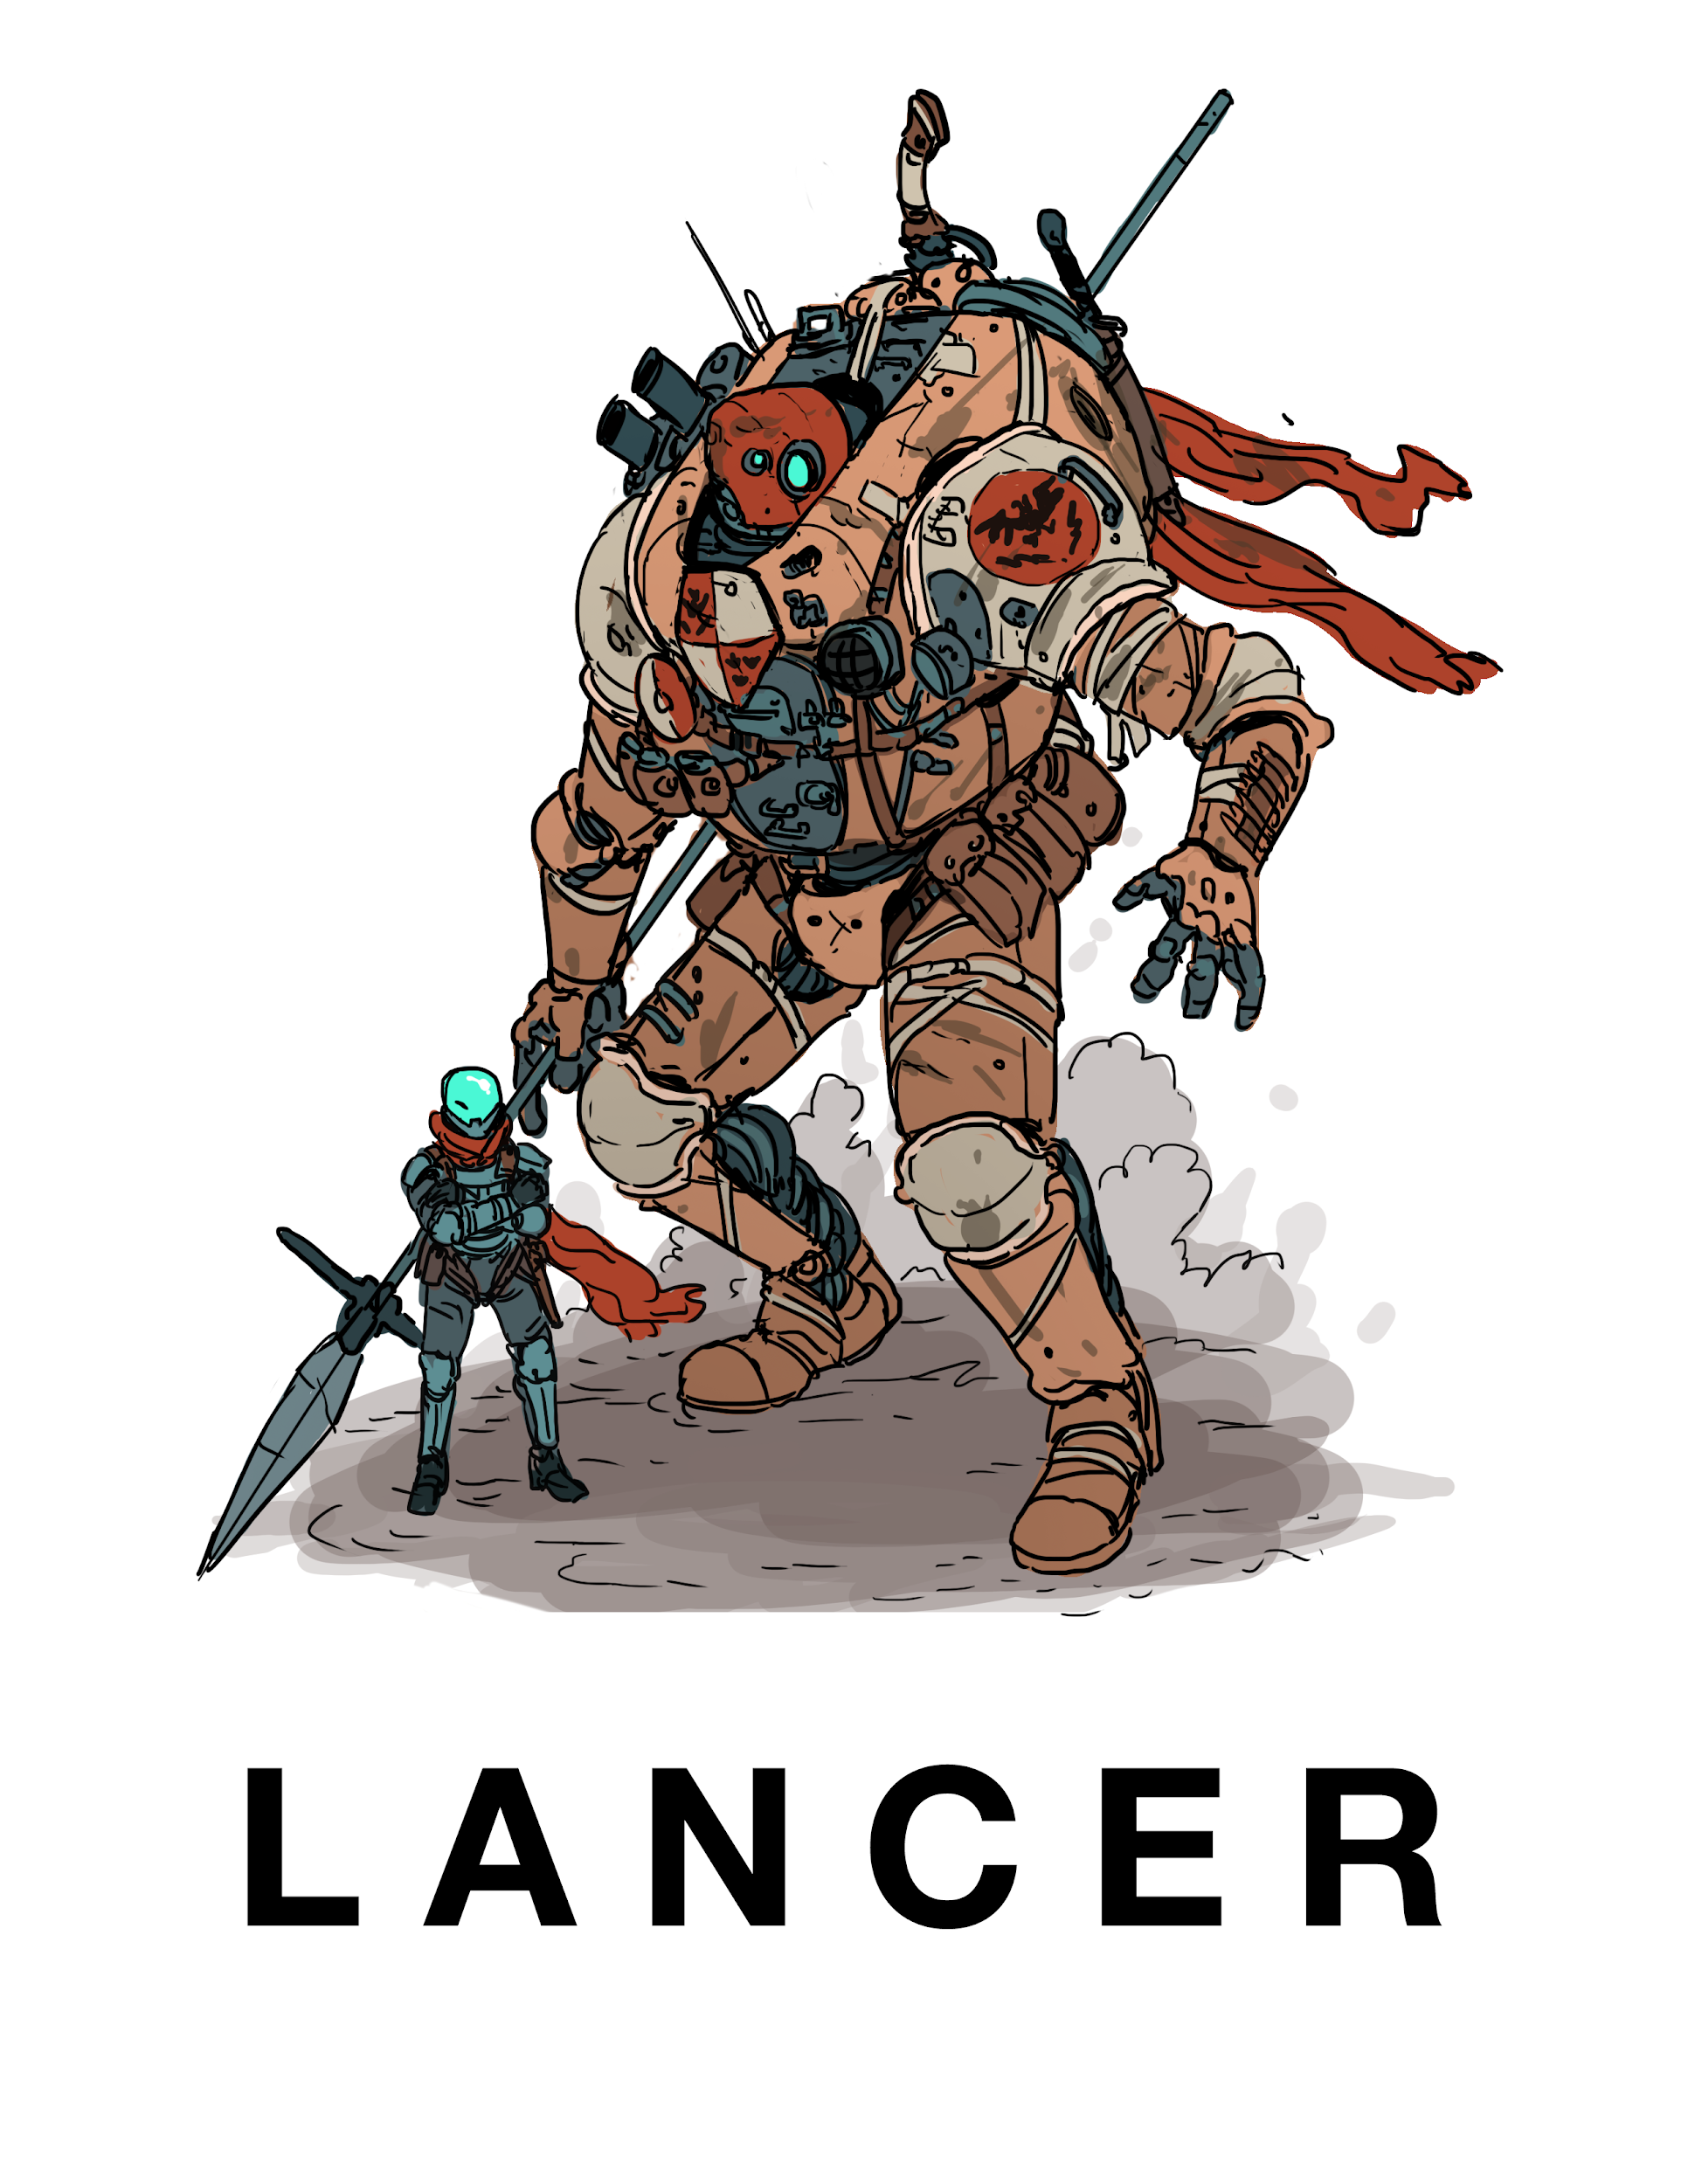
\includegraphics{Cover}
\end{center}

\newpage
\pagestyle{plain}
\begin{titlepage}
\vspace*{\stretch{1.0}}
\begin{center}
\par\noindent\rule[1cm]{0.78\textwidth}{3mm}
{\fontsize{96}{115}\selectfont LANCER}
\vspace{1cm}
\par\noindent\rule{0.78\textwidth}{3mm}
\vfill
\huge\textbf{COMMUNITY EDITION RULEBOOK}
\vfill
\normalsize\textbf{By}

\textbf{Miguel Lopez and Tom Parkinson Morgan}

\textbf{and the Lancer community}
\vfill
1.8 Beta - CE pre-release\\
Please do not reproduce without permission\\
\end{center}
\vspace*{\stretch{2.0}}
\end{titlepage}
\import{./source/}{changelog}

% We set the page number to 2, so the PDF page number = the text page number
\addtocounter{page}{2}

\tableofcontents

\newpage
\import{./source/}{intro}
\import{./source/}{cavalry}
\import{./source/}{basicRules}
\import{./source/}{licenseToKill}
\import{./source/}{pilot}
\import{./source/}{basicStructure}
\import{./source/}{theMech}
\import{./source/}{mechCombat}
\import{./source/}{compendium}
\import{./source/}{theGM}
\import{./source/}{gmToolkit}
\import{./source/}{npc}
\import{./source/}{lore}

\end{document}